% Created 2018-02-06 Tue 22:58
\documentclass[11pt]{article}
\usepackage[utf8]{inputenc}
\usepackage[T1]{fontenc}
\usepackage{fixltx2e}
\usepackage{graphicx}
\usepackage{longtable}
\usepackage{float}
\usepackage{wrapfig}
\usepackage{rotating}
\usepackage[normalem]{ulem}
\usepackage{amsmath}
\usepackage{textcomp}
\usepackage{marvosym}
\usepackage{wasysym}
\usepackage{amssymb}
\usepackage{hyperref}
\tolerance=1000
\date{\today}
\title{Ditigal Transmitters and Recievers}
\hypersetup{
  pdfkeywords={},
  pdfsubject={},
  pdfcreator={Emacs 25.3.1 (Org mode 8.2.10)}}
\begin{document}

\maketitle
\tableofcontents

\section{Lecture 1 - History of Communication}
\label{sec-1}
This is mt, I have not a copy of these notes. Mainly discussed how in the last 120 years we/society has gone from using semophores to using modern fast as light coms.
\section{Lecture 2 - A cont. of lecture 1}
\label{sec-2}
More info I don't have a copy of\ldots{}.
\section{Lecture 3}
\label{sec-3}

\section{Lecture ?}
\label{sec-4}
:DATE: \textit{<2018-02-05 Mon>}



\subsection{Transmitter}
\label{sec-4-1}
two bits per symbol - four possible wave forms
\begin{center}
\begin{tabular}{rrl}
symbol & bits & four possible waveforms\\
0 & 00 & 0$^{\text{0}}$\\
1 & 01 & 90$^{\text{0}}$\\
2 & 10 & 180$^{\text{0}}$\\
3 & 11 & 270$^{\text{0}}$\\
\end{tabular}
\end{center}

\subsection{Reciever}
\label{sec-4-2}
Use correlators to match input to possible transmitted waveforms

\begin{figure}[htb]
\centering
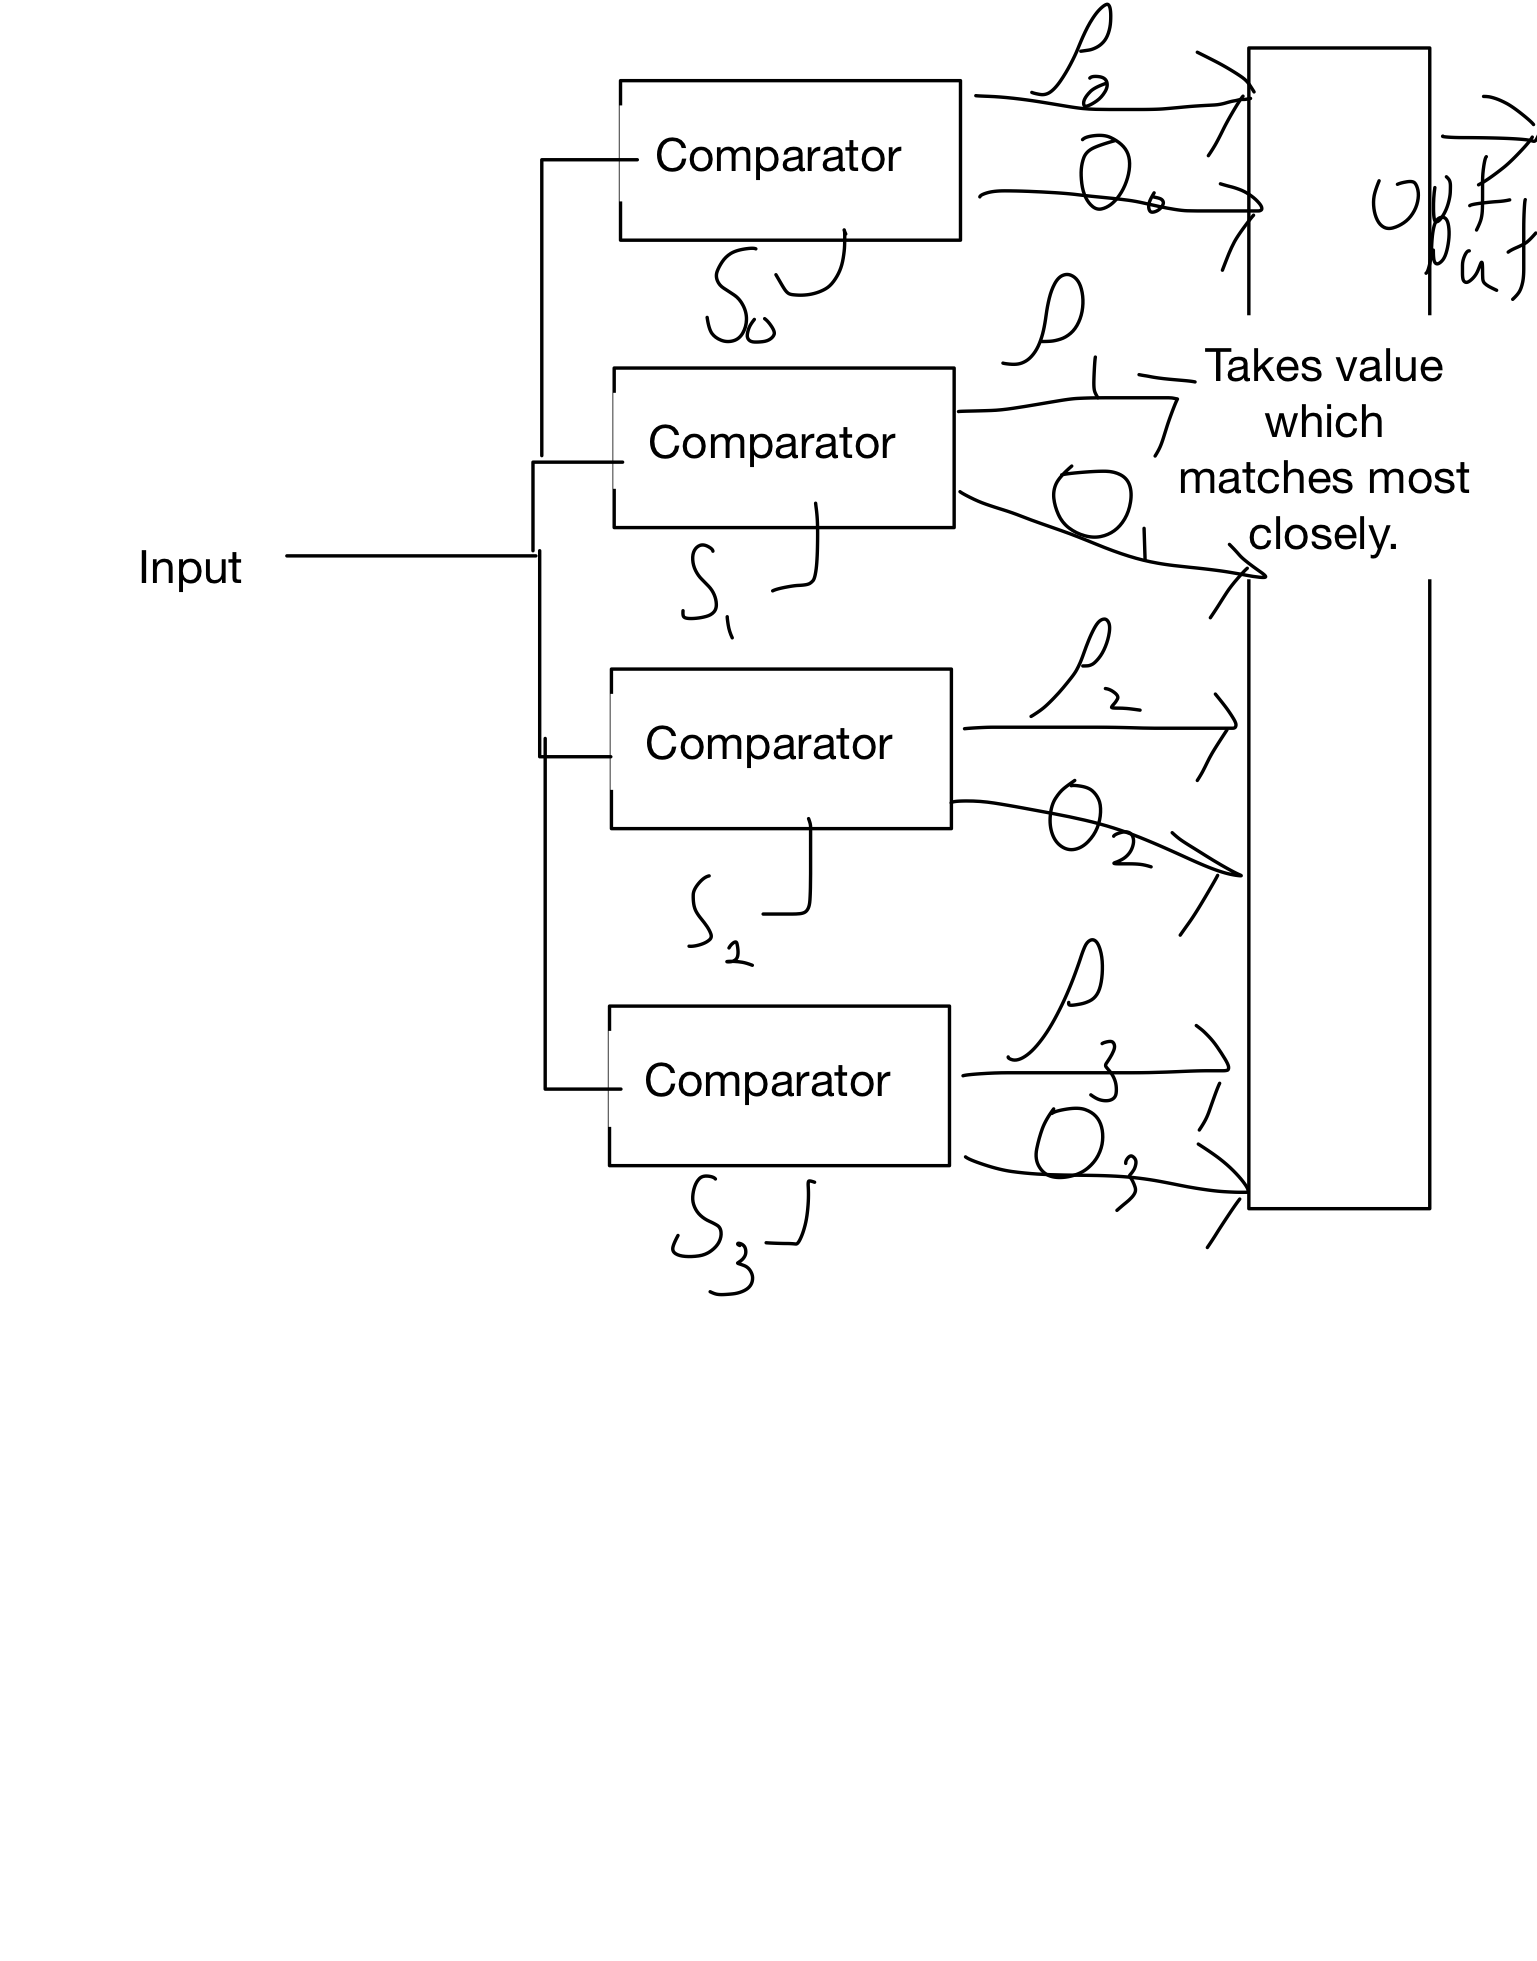
\includegraphics[width=.9\linewidth]{./img/Digital_reciever.png}
\caption{internals of Ditigal reciever with two-bit decode}
\end{figure}

\subsection{{\bfseries\sffamily TODO} Graham-Schmidt: check matrix algebra book on this topic.}
\label{sec-4-3}


\begin{itemize}
\item Signals S$_{\text{1}}$(t),\ldots{},S$_{\text{m}}$(t)
\item basis functions $\phi$$_{\text{n}}$(t),\ldots{},$\phi$$_{\text{n}}$(t), N $\neq$ M
\item \(S_i(t) = \sum{n=1}{N}{S_{in} \phi_n(t)}\)
\item \textbf{S$_{\text{i}}$} = [S$_{\text{i1}}$ S$_{\text{i2}}$ \ldots{} S$_{\text{in}}$]
\end{itemize}

\subsubsection{1st signal}
\label{sec-4-3-1}

E$_{\text{s1}}$ = $||S_{1}||^2$

\$$\phi$$_{\text{1}}$ = $\frac{S_1(t)}{\sqrt{E_{s1}}}$

$S_{11} = \sqrt{E_{s1}}$

\subsubsection{2nd -- Nth signal}
\label{sec-4-3-2}
\emph{Creating a new basis function}

S$_{\text{21}}$ = <S$_{\text{2}}$(t),$\phi$$_{\text{1}}$(t)>



r$_{\text{2}}$(t) = S$_{\text{2}}$(t) - S$_{\text{21}}$ $\phi$$_{\text{1}}$(t) <-- orthogonal to $\phi$$_{\text{1}}$(t)

\texttt{If remainted r\_i(t) = 0 skip the steps below}

\begin{itemize}
\item The part of signal 2 that can't be represented by $\phi$$_{\text{1}}$(t).

E$_{\text{r2}}$ = ||r$_{\text{2}}$(t)||$^{\text{2}}$

$\phi$$_{\text{2}}$(t) = $\frac{r_2(t)}{\sqrt{E_{r2}}}$

S$_{\text{22}}$ = $\sqrt{E_{r2}}$
\item others

S$_{\text{ni}}$ = <S$_{\text{n}}$(t) , $\phi$$_{\text{i}}$(t)> for $\phi$$_{\text{i}}$(t) which are defined.

r$_{\text{i}}$(t) = S$_{\text{i}}$(t) - $\sum$\{S$_{\text{in}}$\} $\phi$$_{\text{n}}$(t)
\end{itemize}

\subsection{Fourier Transfrom}
\label{sec-4-4}

\begin{itemize}
\item \textbf{F} \{g(t)\} = G(f) = $\int_{-\inf}^{\inf} g(t) e^{-j2\pi ft}$

\item \textbf{F} $^{-1}$ \{G(f)\} = g(t) = $\int_{-\inf}^{\inf} G(f) e^{j2\pi ft}$
\end{itemize}


\subsubsection{{\bfseries\sffamily TODO} Properties: verify that \ref{EQ1} is correct}
\label{sec-4-4-1}
\begin{itemize}
\item Linearity
\begin{itemize}
\item \textbf{F} ${a_1 x_1(t) + a_2 x_2(t)}$ = a$_{\text{1}}$ \textbf{F} ${x_1(t)}$ + a$_{\text{2}}$ \textbf{F} ${x_2(t)}$
\end{itemize}
\item Time Shift
\begin{itemize}
\item \textbf{F} ${x(t - T_0)}$ = $\int_{-\inf}^{\inf} x(t-t_0) e^{-j2\pi ft}$

$\lambda$ = t-t$_{\text{0}}$

= $e^{-j2\pi f}\int_{-\inf}^{\inf}{x(\lambda +t_0)}$

= e$^{\text{-j2}\pift_{\text{0}}}$ $\int_{-\inf}^{inf} x(\lambda) e^{-2\pi f\lambda} d\lambda$ \label{EQ1} (EQ1)

= e$^{\text{-2j}\pift_{\text{0}}}$ X(f)
\end{itemize}

\item Frequency Property
\begin{itemize}
\item \textbf{F} $^{-1}{X(f-f_0)} = e^{j2\pi f_0t} \int_{-\inf}^{\inf}{x(t)}$
\end{itemize}
\end{itemize}
% Emacs 25.3.1 (Org mode 8.2.10)
\end{document}
